\chapter{Uživatelská dokumentace}

Aplikace slouží k~vyhledávání receptů pocházejících z~různých webových stránek s~recepty. Aktuálně nabízí recepty ze stránek Food.com a~Allrecipes. Recepty je možné prohlížet přímo v~aplikaci, nechybí ale ani odkazy na zdroj, kde jsou k~dispozici detailnější informace včetně recenzí, doprovodných videí nebo dalších příspěvků autora receptu. Pro vybrané ingredience jsou k~dispozici rozšiřující informace, ke kterým se lze dostat přes detail receptu a~jeho seznam surovin.

\section{Vyhledávání receptů}

Při otevření domovské stránky aplikace na adrese \texttt{/recipes} se zobrazí všechny recepty, kterých je v~současnosti přibližně $91\,000$. Vzhled domovské stránky je znázorněn na obrázku \ref{obr05:homepage}. Recepty jsou vždy zobrazovány po stranách s~maximálně $24$ výsledky. Celkový počet stran není nijak omezen, jako tomu je u~řady jiných webových aplikací. Postupným listováním lze tedy získat všechny recepty, což je viditelné na obrázku \ref{obr05:pagination}.

\begin{figure}[h!]\centering
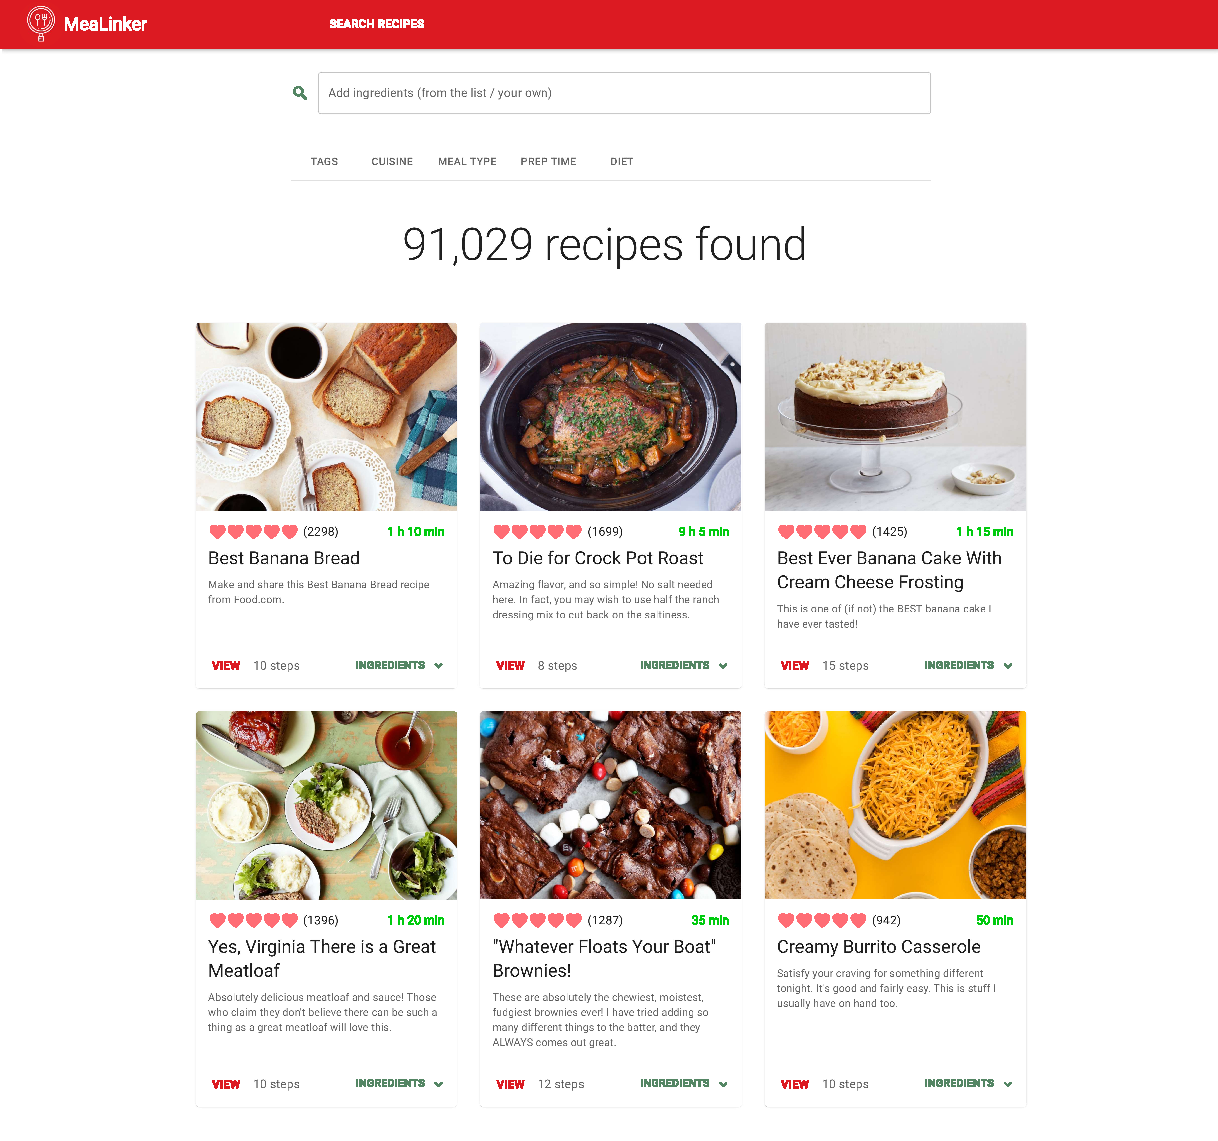
\includegraphics[width=140mm]{../img/homepage}
\caption{Domovská stránka aplikace s vyhledáváním bez zadaných filtrů.}
\label{obr05:homepage}
\end{figure}

\begin{figure}[h!]\centering
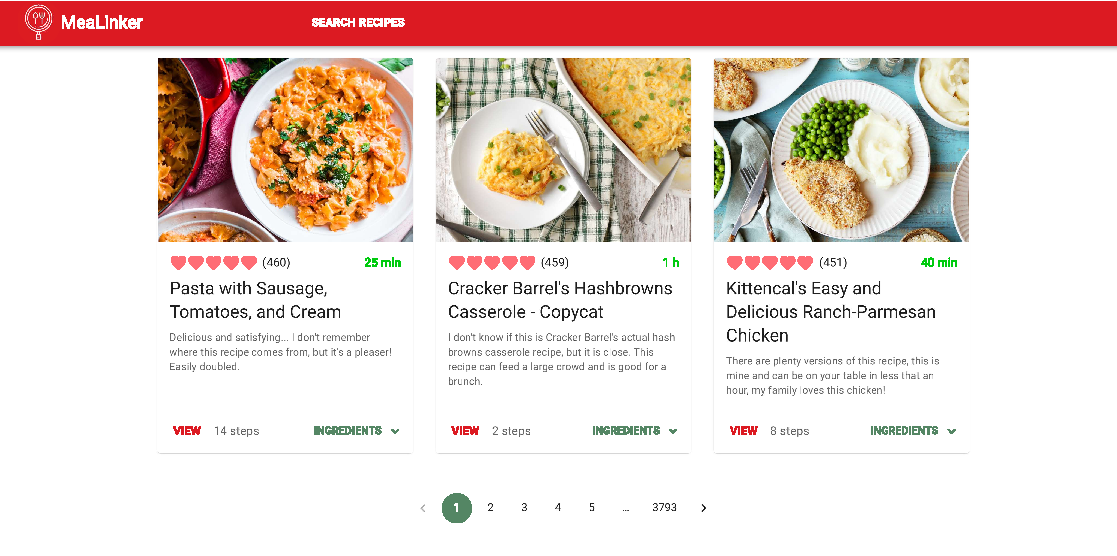
\includegraphics[width=140mm]{../img/pagination}
\caption{Stránkování zpřístupňující všechny nalezené recepty.}
\label{obr05:pagination}
\end{figure}

Aplikace umožňuje vyhledávání receptů upřesnit na základě různých kritérií. Největší důraz je kladen na vyhledávání podle ingrediencí, v~nabídce je ale také filtrování pomocí klíčových slov, kuchyně, typu pokrmu, času přípravy a~diety. Filtry lze libovolně kombinovat a~pro lepší orientaci je u~každé hodnoty napsán počet receptů, které se po přidání tohoto filtru zobrazí. Tomuto stylu vyhledávání se říká fasetová navigace.

Filtry se vždy zobrazují na dvou místech --- v~původním formuláři, do kterého byly vyplněny, ale také pod nadpisem s~počtem vyhledaných receptů. Zde jsou shromážděné filtry ze všech kategorií a~pomocí tlačítka s~ikonou koše je lze snadno odstranit všechny najednou, viz obrázek \ref{obr05:filter-search}. Filtry lze odstranit na libovolném z~těchto míst a~změna se okamžitě projeví i~na místě druhém. Každá změna filtru, ať už přidání nového nebo odebrání stávajícího, spustí automatické vyhledávání receptů. U~filtrů kuchyně a~času přípravy nelze zadat více hodnot najednou.

\begin{figure}[h!]\centering
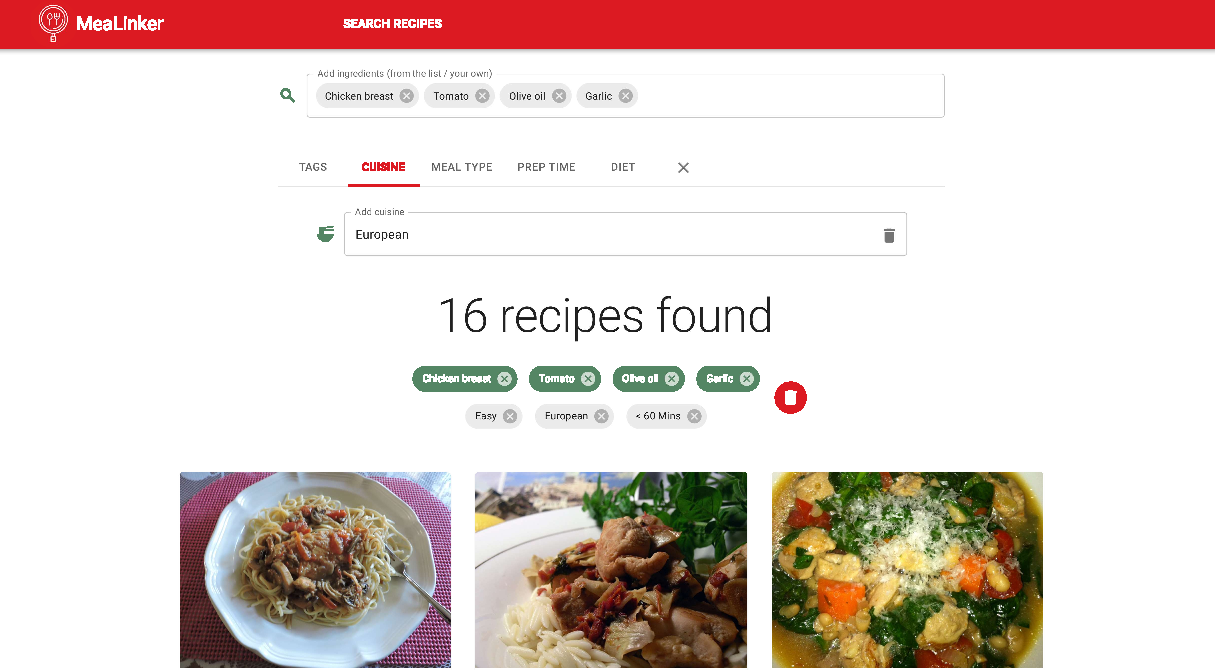
\includegraphics[width=140mm]{../img/filter-search}
\caption{Vyhledávání dle surovin, kuchyně, času přípravy a složitosti.}
\label{obr05:filter-search}
\end{figure}

Pro snadnější orientaci v~nalezených výsledcích lze u~každého receptu rozbalit seznam ingrediencí. V~tomto seznamu jsou zvýrazněny aktuálně vyhledávané ingredience, viz obrázek \ref{obr05:expanded-ingrs}. Seznam je zobrazován přes kartu receptu o~řádek níže a~jeho zavření je potřeba vyřešit ručně kliknutím na ikonu šipky, případně pokračovat na další stranu výsledků.

\begin{figure}[h!]\centering
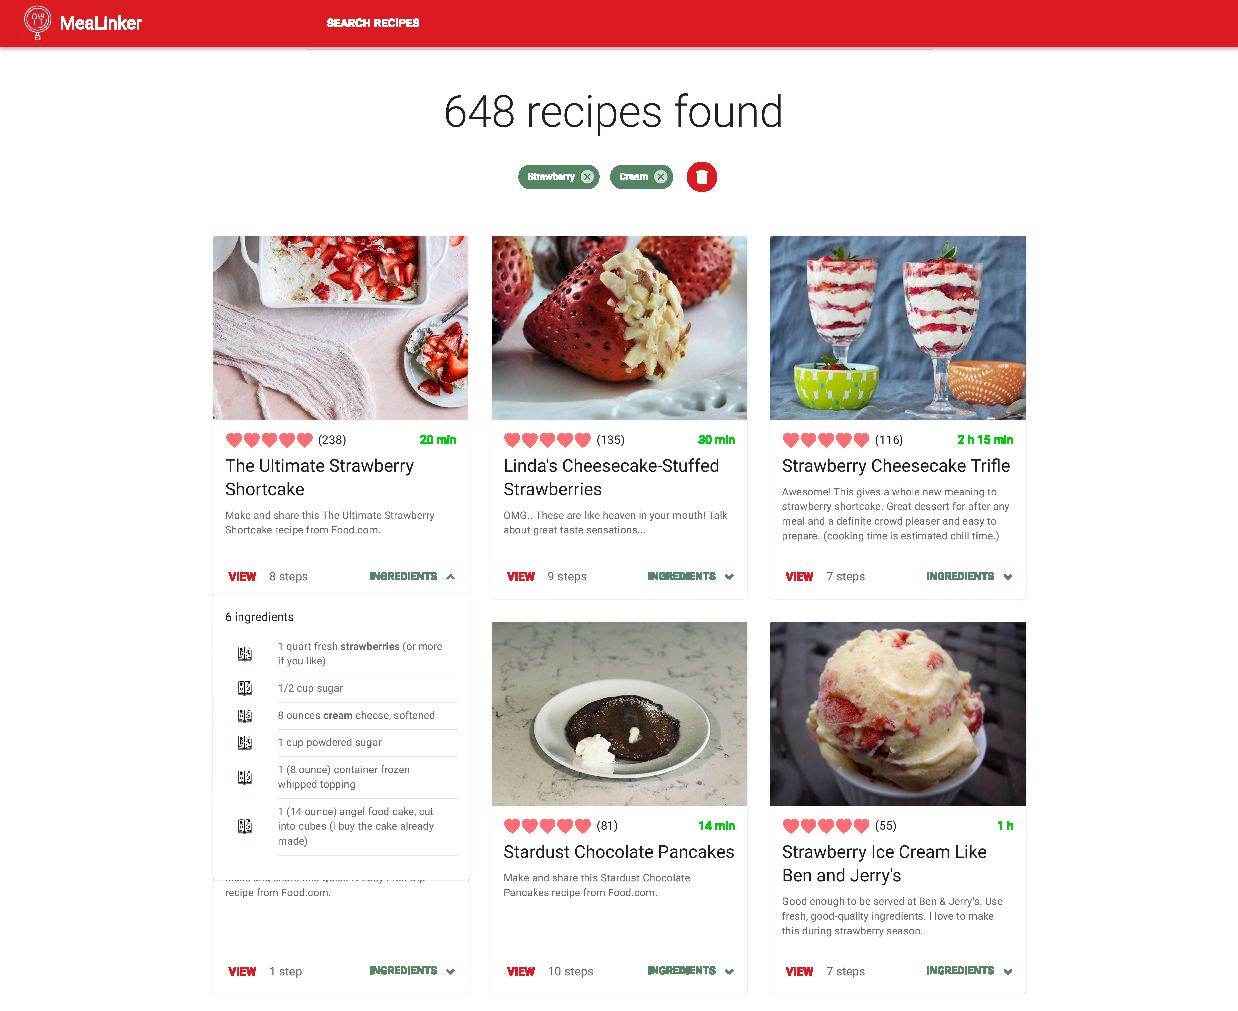
\includegraphics[width=140mm]{../img/expanded-ingrs}
\caption{Rozbalený seznam ingrediencí receptu.}
\label{obr05:expanded-ingrs}
\end{figure}

\section{Detail receptu}

Na obrazovce s~detailem receptu lze vyčíst všechny potřebné informace pro přípravu receptu včetně ingrediencí a~postupu přípravy, viz obrázek \ref{obr05:recipe-detail}. Také je zde k~dispozici tabulka s~nutričními hodnotami. Vybrané ingredience jsou barevně zvýrazněny, což naznačuje, že jsou u~nich k~dispozici rozšiřující informace. Na tyto ingredience lze kliknout, čímž se otevře stránka s~detailem ingredience.

Obrázek receptu je možné přibližovat a~oddalovat pomocí příslušných tlačítek v~levém horním rohu nad fotografií, ale také pomocí touchpadu nebo přidržením klávesy \texttt{Ctrl} a~kolečka myši. Rychlé přiblížení funguje i~přes dvojklik myši. V~pravém horním rohu nad obrázkem je vždy odkaz na zdrojovou stránku receptu, kde jsou typicky doplňující informace v~podobě recenzí nebo podobných receptů. Aktuální verze aplikace neposkytuje modul recenzí, pro jejich prohlížení nebo přidávání je tedy potřeba navštívit zdrojovou stránku.

\begin{figure}[h!]\centering
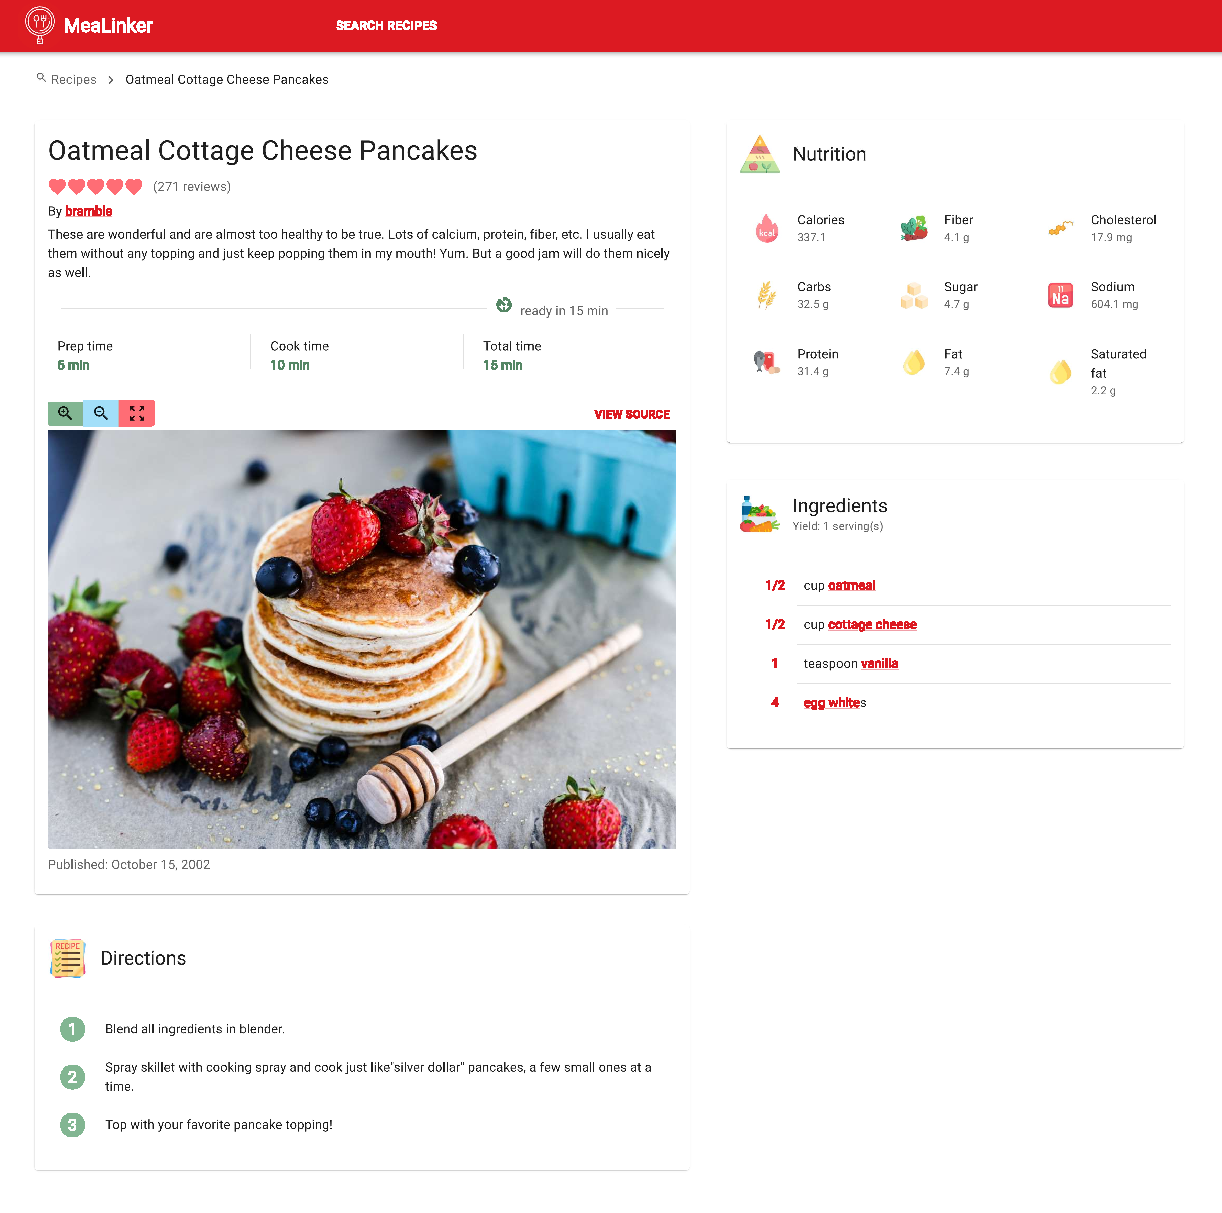
\includegraphics[width=140mm]{../img/recipe-detail}
\caption{Obrazovka detailu receptu.}
\label{obr05:recipe-detail}
\end{figure}

\section{Detail ingredience}

Obsah a~design obrazovky ingredience je proměnlivý podle množství informací, které se k~dané surovině podařilo získat. Standardně obsahuje název, obrázek, popis a~odkaz na zdroj (typicky Wikipedie). Dále volitelně nutriční hodnoty a~kategorie, obojí lze nahlédnout z~obrázku \ref{obr05:ingredient-detail}. Kategorie se dělí na $2$ typy:
\begin{itemize}
    \item Statické kategorie, které mají pouze informativní charakter a~nelze s nimi nijak interagovat, neboť obsahují jen aktuální ingredienci. Jsou označeny světle šedou barvou --- příkladem je kategorie \texttt{Pedaliaceae} na obrázku \ref{obr05:ingredient-detail}.
    \item Rozbalovací kategorie, které obsahují aspoň $1$~ingredienci odlišnou od aktuální ingredience. Přísady uložené v~těchto kategoriích mají výraznější zelenou barvu (viz obrázek \ref{obr05:ingredient-categories}) a~kliknutím je lze otevřít.
\end{itemize}

\begin{figure}[p]\centering
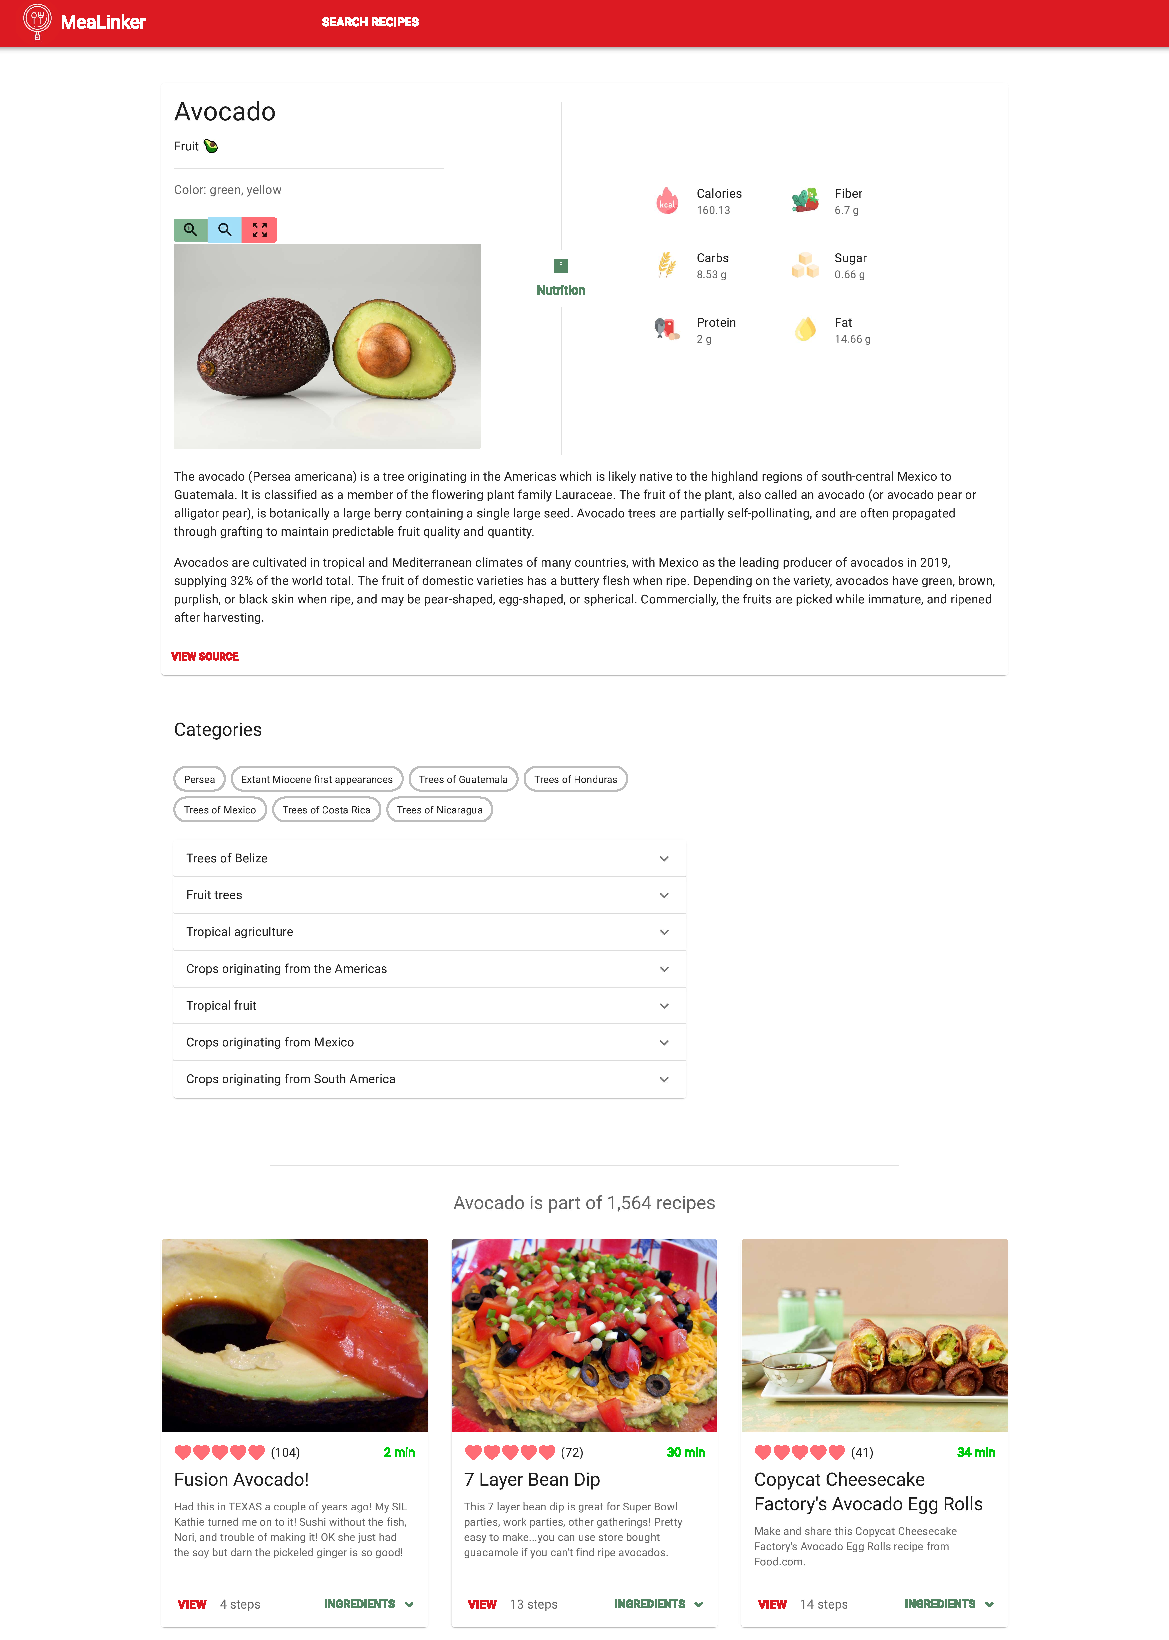
\includegraphics[width=140mm]{../img/ingredient-detail}
\caption{Obrazovka ingredience s~nutričními hodnotami a~kategoriemi.}
\label{obr05:ingredient-detail}
\end{figure}

Pokud se jedná o~takzvaně složenou ingredienci, tak lze na stránce najít přísady, ze kterých je tato ingredience vyrobená. Tato informace je prezentována ve vnořené kartě s~názvem \texttt{Made\,of}. Příkladem je ingredience \texttt{Guacamole} (obrázek \ref{obr05:ingredient-categories}), kterou je možné vyrobit ze základních ingrediencí avokáda, cibule, limetky, soli a~koriandru. U~některých surovin je pod názvem uvedeno místo původu, jak je možné vidět opět na obrázku \ref{obr05:ingredient-categories}. Pod informacemi k~ingredienci následují karty receptů obsahující aktuální ingredienci. Rozložení karet je identické s~vyhledávací obrazovkou receptů a~rovněž je zde možné prohlížet více stran výsledků. 

\begin{figure}[h!]\centering
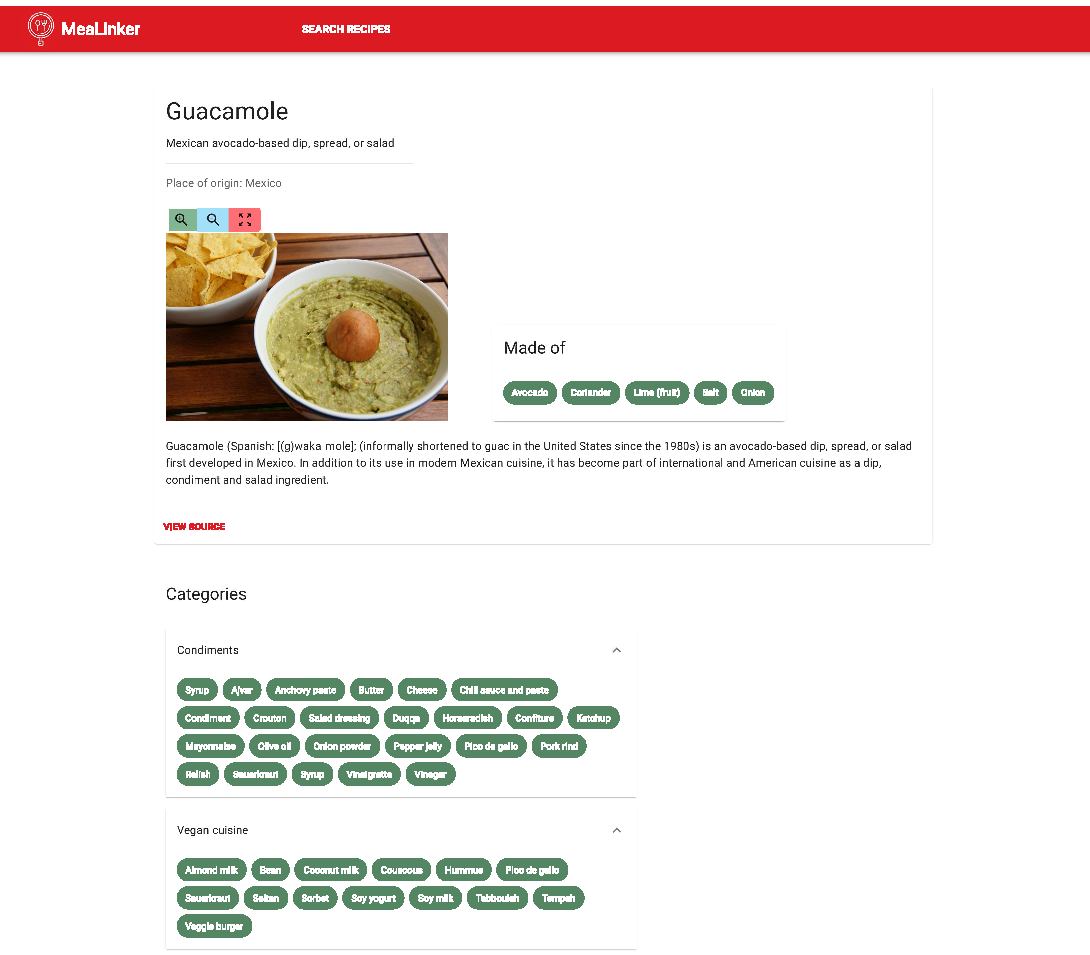
\includegraphics[width=140mm]{../img/ingredient-categories}
\caption{Obrazovka detailu ingredience s rozbalenými kategoriemi.}
\label{obr05:ingredient-categories}
\end{figure}